\chapter{Analysis of Related Work} \label{analysis}

In this chapter we summarize the work done by other authors which is related to the topic of this thesis. At first, we summarize the algorithms which have been developed for subgraph isomorphism matching and their comparison. Next we describe indices which might be used for obtaining the candidate set and algorithms which are used for their construction. The next part of this chapter focuses on approaches which utilize query mechanisms of particular relational and graph databases. In the last part we provide a summary of commercially used solutions.\\

\section{Subgraph Isomorphism Algorithms}

This section does not provide in-depth comparison of available algorithms since it is not a main topic of this thesis.\\

Almost all papers related to subgraph query methods refer two algorithms - Ullmann \cite{Ullmann} and VF2 \cite{VF2}. Those two algorithms are deeply compared in the \cite{Ehrlich2012} benchmark where VF2 outperforms Ullmann.\\

In paper \cite{Lee} there is a comparison of four algorithms derived from Ullmann's algorithm. These are VF2, QuickSI \cite{QuickSI}, GraphQL \cite{GraphQL}, GADDI \cite{GADDI} and SPath \cite{SPath}. They were compared using three real-world data sets. Although all three comparisons have a different winner, it seems that the most efficient algorithm is QuickSI in an average use-case.

\section{Index Building Methods}

In the first part of this section we briefly describe algorithms for building indices on top of chemical compound databases. These are \textit{GraphGrep} \cite{GraphGrep}\cite{GrahGrep:intro}, \textit{GIndex} \cite{GIndex}, \textit{GString} \cite{GString}, \textit{GraphGrepSX} \cite{GraphGrepSX}, \textit{GIRAS} \cite{GIRAS}, \textit{C-tree} \cite{CTree} and \textit{GDIndex} \cite{GDIndex}\\

They form just a selection from a much bigger set of applicable methods and they were picked for different reasons:

\begin{itemize}
	\item The method is mentioned in a majority of relevant articles
	\item The method uses an original algorithm or data structure
	\item The method has excellent results in benchmarks
\end{itemize}

Some of them can be used in generic graph databases, some of them are very specific to the field of chemical compounds but with some effort they might be used also for other graph databases with a specific point of interest.\\

In the following sections we will briefly introduce the basic ideas behind all the previously mentioned methods.

\subsection{GraphGrep}

Very simple and intuitive indexing technique which can be used in any graph database with labeled graphs is called \textit{GraphGrep}. The presumption is that every vertex has a defined unique ID.\\

For each graph in the database there is a constructed index represented as a hash table where the key is a hashed value of a \textit{label-path} (a concatenation of the vertex/edge labels on the path) and the value is a number of unique \textit{id-paths} (a concatenation of the vertex IDs on the path) which represent a particular \textit{label-path} in the graph. In the hash table there are all \textit{label-paths} which are present in the graph up to length \textit{l}, where \textit{l} is a parameter. This hash table is called a \textit{graph fingerprint}.\\

For example the graph in Figure~\ref{fig:graphgrep} would be represented in the index with $l=3$ as depicted in Table \ref{tab:graphgrep}. The numbers in the picture represent the vertex ID, characters next to each vertex represent its label.

\begin{figure}[h]
	\centering
	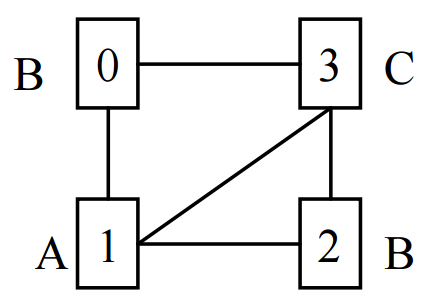
\includegraphics[width=0.25\textwidth]{../img/graphgrep.png}
	\caption{GraphGrep example graph}
	\label{fig:graphgrep}
\end{figure}

\begin{table}[h]
	\centering
	\renewcommand{\arraystretch}{2.5}
	\setlength{\arrayrulewidth}{0.5mm
	}
	\begin{tabular}[h!]{|p{3cm} p{3cm}|p{3cm} p{3cm}|}
		\hline
		\rowcolor{lightgray}
		Key & Value & Key & Value\\ \hline
		h(A) & 1 & h(ABC) & 2\\
		h(B) & 2 & h(ACB) & 2\\
		h(C) & 1 & h(BAC) & 2\\
		h(AB) & 2 & h(BCA) & 2\\
		h(AC) & 1 & h(BAB) & 2\\
		h(BA) & 2 & h(BCB) & 2\\
		h(BC) & 2 & h(CBA) & 2\\
		h(CA) & 1 & h(CAB) & 2\\
		h(CB) & 2 & & \\ \hline
	\end{tabular}
\caption{GraphGrep example graph fingerprint}
\label{tab:graphgrep}
\end{table}

The same process is used for the query. The query itself is also a graph and therefore the hash table can be created too. Then, in the candidate set creation part, each graph’s fingerprint is compared to the query fingerprint.\\

If any value in the query fingerprint is higher than value in the graph fingerprint for the same key or when some key from the query fingerprint is missing in the graph's fingerprint, it means that this graph can be filtered out from the candidate set because we know that the query cannot be its subgraph.

\subsection{GraphGrepSX}

GraphGrepSX is an improved version of GraphGrep. It uses the very same approach for obtaining all the indexed features - it takes all the paths up to the length $l$ from all the graphs in the database. The core of the improvement is in the data structure where the index is stored.\\

Storing all the paths for each graph in a hash table is quite ineffective. Most of the paths appear in more than one graph and we do not need to store these duplicate keys more than once.\\

This method stores the paths in the suffix tree instead. Each node in the suffix tree represents a path (which is an extension of its parent) and contains a set of pairs $(graph, count)$ where $graph$ is an ID of the database record and $count$ is the number of occurrences of the represented path in the $graph$.\\

The way how the query is processed is very similar to the GraphGrep. It mines all the paths up to length $l$ from the query graph and finds the matching nodes in the index tree. For each matched node we need to check whether the number of occurrences for each graph is equal or higher than the number of occurrences in the query graph. If so, we can add this database record into the candidate set. If some path from the query graph is not in the index, we can return an empty candidate set.

\subsection{GIndex}

This method utilizes the concepts of \textit{frequent subgraphs} and \textit{discriminative fragments}. It also comes with an innovative data structure for storing the index.\\

Since the number of all subgraphs grows exponentially with the size of the graph and therefore it would be impossible to index all of them, we need to prune the number of index records to be as compact and still as efficient as possible.\\

Because of the mentioned reasons the \textit{frequent subgraphs} and \textit{discriminative fragments} concepts have a significant role.\\

\textbf{Frequent subgraphs} are all subgraphs which are contained in at least \linebreak $ minSup $ (minimum support) graphs in the database. The survey of frequent subgraph mining can be found in \cite{frequentGraphs}. Suppose we have an index from all frequent subgraphs and for each record in the index we have a set of IDs of graphs in the database in which it occurs. If the query graph $ q $ is frequent, we have the candidate set immediately. If not, we can get the candidate set as an intersection of matched graphs sets of all frequent subgraphs of $ q $.\\

Utilization of pure set of frequent subgraphs with static $ minSup $ attribute has a couple of issues. With $ minSup $ set too low, we get an enormous set of frequent subgraphs. If the $ minSup $ is too high, the candidate set can be too large (at least $ minSup $) with larger probability of false positives.\\

That is why the described method comes with size-increasing support function. It is a non-decreasing function which takes the graph size as an argument (defined as the number of edges) and returns the $ minSup $ for given size. This results in smaller $ minSup $ for small graphs (because of the efficiency) and bigger $ minSup $ for large graphs (because of the compactness). To prevent too big subgraphs in the index, it is necessary to specify a threshold starting from which the function returns infinite.\\


An additional pruning of the index can be done. There is a very high chance that frequent subgraph $ g $ will not be enough discriminative. It means that  the candidate set of $ g $ is not significantly smaller than the intersection of candidate sets of its subgraphs.\\

\textbf{Discriminative fragments} concept brings a new metric. It measures how much discriminative the frequent subgraph is in comparison to the set of its subgraphs in the index. The discriminative ratio is defined as

$$ \gamma = \frac{|\bigcap _{i} D_{f_{\varphi i}} |}{| D_{x} |} $$

\noindent where $D_{x}$ is the set of graphs containing $ x $ and $ D_{f_{\varphi i}} $ is the set of graphs which contain subgraphs of $ x $ which are in the index. If the discriminative ratio is close to 1, we know that the discriminative power is low.\\

\textbf{gIndex} is a prefix tree data structure. Its nodes are of 2 types - \textit{discriminative} and \textit{redundant}. Each node’s key is a text string which represents the subgraph. It is serialized and canonized based on special application of DFS algorithm. This technique is called \textit{DFS Coding} and is described in \cite{gspan}.\\

Discriminative nodes are both frequent (based on given \textit{size-increasing support function}) and discriminative (based on specified $ \gamma $) and they contain a list of IDs of all graphs in the database which contain the particular subgraph. Redundant nodes are present just to satisfy the structure of the \textit{gIndex} tree.\\

The root of the tree is an empty graph, whose candidate set is the whole database. Level 1 of the tree is the set of vertices (graphs of size 0). Each node in the tree (from level 2) has 1 more edge than its parent (because of the canonization it has its parent’s key as its prefix).\\

It would be very inefficient to check all subgraphs of a query graph. But, we know that if subgraph $ g $ is not present in graph $ G $, then no superstructure of $ g $ is present in $ G $. Also, we know that if $ g $ and $ h $ are subgraphs of $ G $ and $ g \subset h $, then the candidate set generated by $ h $ is a subset of candidate set generated by $ g $ and therefore it has a bigger pruning power and usage of $ g $ is redundant.\\

From the two previously mentioned statements it is apparent what is the search algorithm. We need to enumerate all fragments of query graph $ q $ starting from 1-node fragments and iteratively enlarge the fragments by adding 1 edge each time. We stop this process at the point where the fragment is not in the index anymore.\\

Each of the fragments which were created in the last iteration can be found in the index. We only need to check whether the matched node in the index is discriminative or redundant. If it is redundant, we find the closest discriminative node on the path to root. Having the set of matched discriminative nodes in the tree, we compute an intersection of their sets of matched graphs in the database to get the desired candidate set.

\subsection{GIRAS}

As \textit{gIndex} comes with an idea of indexing frequent and discriminative fragments, GIRAS indexes rare and discriminative fragments. The idea is to get higher pruning power and put the indexing focus on the graph features which are specific for a particular record in the database. Ultimately, to have a unique index for each graph in the database. This leads to much smaller index size.\\

For getting the rare fragments it utilizes the modified version of \textit{gSpan} algorithm \cite{gspan}. Although, the original \textit{gSpan} is designed to get all subgraphs whose support in the database is \textit{n or higher}, the modified version finds all the subgraphs whose support is equal to \textit{n}.\\

The modified \textit{gSpan} utilizes minimal DFS codes which were already described in \textit{gIndex} section. It starts with an empty DFS code and in each call it finds all the possible right-most extensions from the whole database. For all of them it finds out whether they are minimal DFS codes and, if so, it checks what the support of this subgraph is. If it is equal to the specified support $f$, the subgraph is added into the result set. If the support is higher, we continue recursively.\\

Note that it returns only the minimal rare substructures with a given frequency. This is important since the extensions of these minimal rare substructures with the same frequency would not give us any more pruning power but it would increase the index size significantly.\\

The GIRAS itself then calls the modified gSpan. It starts for $f=1$. After each call of modified gSpan it checks which database records are represented by the result set of gSpan. If there are database records which are not indexed yet, the modified gSpan is called iteratively with $f+1$. Once there are all database records indexed, we are finished. The last $f$ is called $f_{min}$ and it is the threshold defining the meaning of rare substructure.\\

Although it is not discussed in the paper \cite{GIRAS} what data structure it uses for the index representation, we found out from the source code obtained from Dr. Azaouzi, the author of the described research, that it uses very similar data structure which was described in \textit{gIndex} section, as well as the same technique for the querying process.

\subsection{GString} \label{gstring}

All other methods can be used in any graph database. On the other hand, GString method is very specific for the organic chemical databases (but can be internally modified to support different graph databases with specific content).\\

The main ideas come from the knowledge of common structures of the graphs in the database. The chemical compounds consist of 3 types of semantic structures - paths, cycles and stars (a central node with a fan-out). Each chemical compound can be converted into a graph whose nodes are not atoms but one of the mentioned structures. This converted graph is significantly smaller than the original one.\\

The other observation is that we can omit the hydrogens since their number can be easily computed and we can omit the labels of carbon atoms and single (saturated) bonds.\\

Based on previous preliminaries, each graph in the database can be shrinked to the graph of common structures. Each node contains 3 types of information:

\begin{itemize}
	\item \textbf{Type} - path, cycle or star
	\item \textbf{Size} - For path and cycle it is the number of nodes, for star it is the fan-out
	
	\item \textbf{Triple} $ <n_{n}, n_{b}, n_{e}> $ where:
	\begin{itemize}
		\item $ n_{n} $ is the number of non-carbon atoms
		\item $ n_{b} $ is the number of branches (connected paths of the length 1)
		\item $ n_{e} $ is the number of double or triple bonds
	\end{itemize}
	
\end{itemize}

For each such graph we can get a set of all paths up to length $ l $. The index structure of GString method is a suffix tree of these paths, where each node is identified by tuple $ <Type, Size> $ and contains a set of pointers to the \textit{detail table} where quadruples $ <n_{n}, n_{b}, n_{e}, id> $ are stored for matched nodes from a particular graph. The suffix tree is built from all paths up to length $ l $ from all graphs in the database.\\

The candidate set is obtained as follows. The query graph itself is translated to the common structure graph by the same process which was utilized for index building. Then we just identify suffix tree nodes which were visited and use the pointers to the \textit{detail table} in such nodes. The graph is added into the candidate set if it is represented in each visited suffix tree node and if the triple $ <n_{n}, n_{b}, n_{e}> $ satisfies the query.\\

It means that for cycles, the $ n_{n} $ and $ n_{e} $ has to be equivalent in both query and database record, $n_{b}$ has to be equal or lower in the query comparing to the database record. For the paths and stars all three attributes has to be same or lower in the query.\\

Note that the answer set of this method can be different from previous methods. Let us take a path of four carbons $ c-c-c-c $ as an example of a query and assume that the benzene (cycle of six carbons) is a part of the database. The previous methods marks the benzene as a \textit{match}. On the other hand the GString will filter it out from the candidate set because it finds out that its \textit{common structure} graph is completely different.\\

However, this is a correct behavior for the chemical compound database since we can expect that if somebody asks for a path of four carbons, he or she does not expect a benzene as a result since cycles and paths have different semantics.

\subsection{C-Tree}

Contrary to the previous methods, this one does not utilize the fragments of the graph to find the candidate set. It builds the state-of-the-art tree structure where the nodes are \textit{closures} of their children so they contain the same substructures as their whole subtrees. Also it comes with the term of \textit{pseudo sub-isomorphism} which is similar (and weaker) to subgraph isomorphism but it can be verified in polynomial time.\\

The core of the C-tree method are the graph closures. Let $ G $, $ G' $ be graphs and $ m $ be the mapping between them (graphs can contain dummy nodes for enabling mapping between graphs of different size). Let $ v $, $ v' $ be nodes from $ G $ or $ G' $, respectively and let $ m(v) = v' $. Vertex closure which corresponds to $ v $ and $ v' $ then contains a union of labels of $ v $ and $ v' $. The very same approach is used for edges.  Let $ e $, $ e' $ be edges from $ G $ or $ G' $, respectively and let $ m(e) = e' $. Edge closure which corresponds to $ e $ and $ e' $ contains a union of labels of $ e $ and $ e' $. \textbf{Graph closure} of graphs $ G $ and $ G' $ is a tuple $ (VC, EC) $ where $ VC $ is a set of vertex closures and $ EC $ is a set of edge closures. Note that $ G $ and $ G' $ can be both graphs and graph closures.\\

Several approaches how to get the mapping $m$ are described in \cite{CTree} and we will not describe these in the this section to not dive too deep into the technical details.\\

The \textbf{C-tree} data structure is a tree where leaf nodes are graphs from the database and every internal node is a graph closure of its children. Each node has at least $ m $ children unless it is root, $ m \geq 2 $, and each node has at most $ M $ children, $ \frac{M+1}{2} \geq m $. All operations with the tree are done in polynomial time and their implementation is analogous to those on R-trees \cite{RTrees}\\

The idea of the method is to approximate the subgraph isomorphism by a weaker statement, \textbf{pseudo subgraph isomorphism}, which can be tested in polynomial time. An important note is that pseudo subgraph isomorphism can be tested on both graphs and graph closures.\\

Full description of the theory behind the pseudo subgraph isomorphism would be too exhaustive for the purposes of this thesis. Very briefly, the idea is to construct a bipartite graph $G$ between vertices of graph $G_{1}=(V_{1}, E_{1})$ and vertices of $G_{2}=(V_{2}, E_{2})$. There is an edge between $v \in V1$ and $u \in V2$ if \textit{breadth-first search tree} around $v$ with the paths up to the specified length $n$ is isomorphic to the one around $u$. If $G$ has a semi-perfect matching, $G_{1}$ is \textit{level-n pseudo subgraph isomorphic} to $G_{2}$\\

The authors of C-tree are also proposing a recursive algorithm which can effectively obtain the information whether two nodes should be connected by an edge in the previously mentioned bipartite graph for the level $n$ based on the bipartite graph for the level $n-1$.\\

The candidate set creation process utilizes the C-tree. It goes from the root to leafs and every time it finds out that a query is not pseudo subgraph isomorphic to some node, this node and its subtrees are pruned out. Leafs which are pseudo subgraph isomorphic to the query are added to the candidate set.\\

The main advantage of this method is that contrary to the previous methods, this one does not loose information during the index creation time. It does not count with paths or any other fragments, the closure tree does contain all the information about all the graphs in the database. This helps to increase the level of the pruning during candidate set creation.

\subsection{GDIndex}

This method's approach is quite different to the previous ones. It tries to completely omit the verification step and therefore computationally hard usage of any subgraph isomorphism detection algorithm. It is achieved by all the subgraphs of all database records.\\


It uses two structures in the index:

\begin{enumerate}
	\item Directed acyclic graph (DAG) of all subgraphs. Each node in the DAG represents a specific connected subgraph. Each such node contains also the information whether it refers an actual record in the database. There is a directed edge from node $ N $ to node $ M $ if $ N $ is a subgraph of $ M $, $ N $ contains exactly 1 vertex less than $ M $ and $ N $ is an induced subgraph of $ M $.
	
	\item Lookup hash table of subgraphs. There is a record in the hash table for each node in the DAG. For hashing, the canonical form of the graph is defined. This canonical form is derived from the adjacency matrix.
\end{enumerate}

Both index building and querying is straightforward. To build the index we just take each graph, add it to the DAG and by gradual removing of its vertices we repeat the same procedure for all its subgraphs. In each step we just need to check whether such node already exists in the DAG which we can easily achieve using the lookup table.\\

To reduce the number of subgraphs, the canonization technique is introduced and from all isomorphic subgraphs only one is used in the index. This canonization technique is very similar to the DFS codes described in \textit{gIndex}, however, instead of minimal DFS code it is using maximal adjacency matrix serialization (but both approaches are equally strong and have the same computational difficulty).\\

Querying is even simpler. All we need to do is to create a canonical representation of the query graph and use the lookup table. If the particular record is not present in the index, we know that the candidate set is empty. If there is such node, we recursively iterate through all its descendants in the DAG and find all pointers to the database graphs. Since we are using hash table, we can get false positives. Therefore, for each record in the matched row of a hash table we need to compare the exact canonical code and we will use only the the record which is exact match.\\

The big advantage of this method is that we do not have to do the NP-complete subgraph isomorphism test since we store the subgraphs in the index and we have the canonical representation.\\

What we have found as a missing piece (and there is no information about this case in the paper) is that the query does not have to be an induced subgraph of any node in the database. It can be more sparse. In this case we cannot expect the exact match of the canonical code and therefore we cannot expect any results.\\

The possible solution to fix this problem would be to index all the subgraphs instead of just induced ones. On the other hand that would have serious impact on the index size.

\subsection{Benchmark Results}

\textit{GraphGrep}, \textit{GIndex}, \textit{GString} and \textit{C-Tree} have been compared in \cite{GString}. As the testing data set the AIDS Antiviral Screen Dataset \cite{AIDS} was used. It contains 43 000 molecules with an average number of 25 vertices.\\

All measured metrics except for the speed of index creation had the same winner. The \textit{GString} algorithm outperforms the others in the size of index, accuracy of the candidate data set and the search time.\\

On the other hand, in \cite{GraphGrepSX} we can find the benchmark of the \textit{GraphGrepSX} method which looks like a more generic version of \textit{GString}. While in \cite{GString} \textit{GString} outperforms \textit{CTree} just by few percents, in \cite{GraphGrepSX}  \textit{GraphGrepSX} outperforms the \textit{CTree} by the two levels of magnitude despite larger candidate sets.\\

In \cite{GDIndex} there is a comparison of \textit{GDIndex} and \textit{C-tree} where \textit{GDIndex} significantly outperforms \textit{C-tree} in all measured metrics - the size of index and its construction time and the search time.\\

What we may question is that how \textit{GDIndex} would perform over a database with larger graphs such as the AIDS dataset which was used in experimental parts of all other methods.\\

In \cite{GIRAS} we can find a benchmark of the \textit{GIRAS}, \textit{C-tree}, \textit{gIndex} and couple of other approaches. On the AIDS dataset \textit{GIRAS} outperforms \textit{gIndex} and \textit{C-tree} in all query sizes. In the dataset with bigger graphs, \textit{GIRAS} outperforms the other two methods only in larger query sizes (12 vertices and more).\\

What is not measured in \cite{GIRAS} is the size of index and time needed for index construction.

\section{Database Management Systems Utilization for Subgraph Querying}

Surprisingly we have not found many articles about substructure querying in DBMS using just their native way how to structure data and their specific query language.\\

The first approach \cite{SQL} we found is about the utilization of relational database management system and SQL queries. The second one \cite{Hoksza} is referring about utilizing a graph DBMS, Neo4j \cite{Neo4J}, and its query language Cypher.

\subsection{SQL Substructure Search}

Contrary to typical subgraph matching algorithms which use variations of the depth-first-search algorithm, the authors of \cite{SQL} come with an SQL based solution which utilizes the principles of the BFS.\\

In the database the molecules are described as follows. The database contains 3 tables - molecules, atoms and bonds. The bonds have an extended type column which is a string identifier that identifies bond type and types of both end atoms type (e.g. there is a unique identificator of two carbons connected by double bond).\\

The bond table has three indices built on top of it. The first one is built for bond type which helps us to do efficient filtering, the second one is built for \textit{atom1\_id} column (a reference to the atoms table) which helps us to get all neighbours for each atom. The last index is built based on unique identifier of records in bond table by atom pairs.\\

When the substructure query is obtained, the minimal spanning tree is constructed. The value of each edge depends on the statistics of the database. We can say that the most rare atom-bond-atom edge has the lowest value. Also in this tree we find a root node which has the least valuable edges on it. This spanning tree will help us to construct an efficient SQL query, because thanks to the spanning tree minimality and the root selection the constraints (edges) with the highest probability of failure will be checked first.\\

The query itself uses only the edge table. It starts from the root of the spanning tree. For each edge there is a specification of an extended bond type and specification of a join to other instance of edge table. At the end there are edges which are not a part of a spanning tree.\\

As an example we can use a subgraph query where we want to find all structures which contain $ O=C-N $. The bond $ C-N $ is more rare in the sample database and therefore this bond is described as the first one in the query. The query itself would look as follows:


\begin{verbatim}
SELECT b1.compound_id, b1.atom1_id, b1.atom2_id, b2.atom2_id
FROM bonds b1, bonds b2
WHERE b1.bond_type = "C-N" and
      b2.atom1_id = b1.atom1_id and 
      b2.bond_type = "O=C"
\end{verbatim}

\noindent where $ C-N $ means carbon and nitrogen connected by a single bond and $ O=C $ means oxygen and carbon connected by a double bond.\\

This example is quite simple. On the other, hand we need to build an SQL query which describes the whole \textit{Constrain Satisfaction Problem}. It means that for each pair of bonds, we have to define whether their atoms do or do not have the same IDs.\\

Where it is possible, we can force usage of built indices. For the first edge we should use the index built for the bond type column. For other spanning tree edges we should use the index for $ atom1\_id $ column which literally does the BFS. For edges outside the spanning tree we should use the index built for $ atom1\_id $, $ atom2\_id $ pair since we already know the IDs of both atoms of the edge we need to check.

\subsection{Neo4j Substructure Search}

Hoksza et al. in \cite{Hoksza} describe their case-study of mining the protein graphs. They use the Neo4j graph DBMS to store the protein database and query it by the Cypher language.\\

They found out that the query time is factorial with respect to the number of edges in the query. Beginning from size 15, the queries were impossible to execute in a reasonable time and therefore they recommend the usage of Neo4j only for small subgraph queries.\\

They have also tried to compare their results with results for an SQL database. However, the SQL results significantly outperform Neo4j. But the comparison is not fair enough since the SQL approach used pre-computed neighborhood relations and therefore had a significant advantage in comparison with Neo4j.\\

However, based on this paper we can be pessimistic in case of Noe4j utilization, we should keep in mind that the database had a different structure comparing to our molecule databases which are the target of this thesis. Graphs used in the experiment have an average size of more than 500 edges. On the other hand, typical molecule databases contain significantly smaller graphs and therefore we cannot be sure that the numbers from the mentioned paper can be applied also for such databases.

\section{Commercially Used Solutions}

In this section we introduce three real-world solutions. The first one is the AMBIT project \cite{Ambit} which offers chemoinformatics functionality via REST web services. One of the functionality is, of course, the substructure search. This project represents a standalone solution - the querying is not dependent on any particular database management system.\\

The second solution, JChem Cartridge \cite{JChem}, is an example of an Oracle cartridge \cite{cartridge}. The reason why we picked this cartridge from the set of existing ones is that it has the best results in the benchmark presentation at \cite{benchmarkPresentation}.\\

The third solution, ABCD Cartridge \cite{ABCD}, is a pure commercial one developed by the Johnson \& Johnson company \cite{JJ}. We picked this one because its architecture is well described in \cite{ABCD} despite the software is not publicly available .

\subsection{AMBIT-SMARTS}

AMBIT-SMARTS is a Java based software built on top of the Chemistry Development Kit (CDK \cite{CDK}). It implements the whole SMARTS querying language specification \cite{SMARTS} for querying chemical databases. It uses two indices. Both are in the form of a bitstring which is stored for each record in the database.\\

Each bit in the first bitstring represents whether some structure is a part of the particular record. The structures are of two kinds.\\

The first set of structures is selected automatically based on the database content. It considers each atom’s topological layers. The first topological layer is the atom and all its neighbours. n-th topological layer is the whole (n-1)-th layer and some or all of its neighbours. All such structures up to a selected layer level are recorded. Structures which are a part of at least ~50\% of database records are considered as those which will be represented in the bitstring.\\

The second set of the structures represented in the first index is selected by the database administrator who should be aware of what types of queries are most likely to be used in such database.\\

The second bitstring represents all paths up to length 7. Because the number of these paths is enormous, they are not represented directly in the bitstring, but they are at first hashed and this hashed value is added (by logical OR) to the bitstring. This concept is called \textit{fingerprints} and it is described in \cite{fingerprints}.

\subsection{JChem Cartridge}

The JChem Cartridge is a part of the JChem package from ChemAxon \cite{Chemaxon}. It allows users to build their chemical database in the Oracle database easily. A part of the cartridge contains tools for chemical formats conversion, similarity search and sub-structure search. It also implements functions for SMARTS queries.\\

With regards to the substructure search it filters the database based on the fingerprints which are present for every molecule. It uses the hashed fingerprints similarly to the AMBIT-SMARTS. The keys for hashing are:

\begin{itemize}
	\item All paths in the molecule up to a specified length
	\item The branching points (atoms with degree higher than two)
	\item All cycles
\end{itemize}

\noindent The fingerprint itself is generated based on 3 user-defined parameters:

\begin{itemize}
	\item The length of the fingerprint
	\item The maximum path length (how long paths are used for generating the hash keys)
	\item How many bits are set to 1 for each hash key
\end{itemize}

In the documentation there is stated that for the substructure search the optimal values in most cases should be 512 bits long fingerprints, the maximum path length set to 5 or 6 and the number of bits per hash key set to 2.\\

The cartridge also has a tool for analyzing the efficiency of the fingerprints. As a good metric the idea of \textit{darkness} is used. Darkness is defined as a ratio between numbers 0 and 1 in the fingerprint. The analysis tool provides the user with information about the lowest, average and highest darkness in the database and also provides a distribution. The darkness should be as low as possible, highest values should not exceed 80\%, but best performance is expected under 66\%.

\subsection{ABCD Cartridge}

ABCD is an integrated drug discovery informatics platform developed by the Johnson \& Johnson Pharmaceutical Research \& Development, L.L.C. It consists of a set of algorithms for subgraph isomorphism checking and index building and an interoperability layer, cartridge, for the Oracle database which enables the RDMS to use the algorithms and indices during the SQL query evaluation.\\

For the filtering it uses a set of hashed fingerprints. There are 5 types of fingerprints which are used for each molecule - atom, edge, ring, path and cluster fingerprint. For each type there is a different algorithm which generates the hash keys. Also for each hash key, the number of occurrences of a particular feature is stored.\\

Contrary to AMBIT it does not store the fingerprints for each record in the database. It utilizes the concept of inverted bitstrings.\\

The algorithm proceeds as follows. Every molecule in the database is analyzed and the set of hash keys along with the number of occurrences in that molecule are computed. The information for each key is stored as a triplet $ {h,c,m} $, where $ h $ is the hash code, $ c $ is the number of occurrences, and $ m $ is the ID of the molecule in the database. The list is then traversed and for each unique hash code, $ h $, a series of binary masks, $ M(h,cmin) $, are defined, where $ M(h,cmin) $ contains the IDs of the molecules for which the hash code $ h $ occurs at least $ cmin $ times.\\

For more compact representation of the inverted bitstring there are three types of their representation where $ N $ is the size of database and $ K $ is the number of database records in the matching set:

\begin{itemize}
	\item If $ K < \frac{N}{32} $ then the representation is an array of IDs of database records which belong to the set.
	\item If $ (N - K) < \frac{N}{32} $ then the representation is an array of IDs of database records which do not belong to the set.
	\item Otherwise it is stored as a classing bitstring where n-th bit represents whether n-th record belongs to the set.
	
\end{itemize}


















